\documentclass[aspectratio=169, 10pt]{beamer}

% --- GÓI HỌC THUẬT & FONT TIẾNG VIỆT CHO XELATEX ---
\usepackage{fontspec}
\setmainfont{Arial}
\setsansfont{Arial}
\setmonofont{Consolas}

\usepackage{amsmath,amssymb}
\usepackage{graphicx}
\usepackage{booktabs}
\usepackage{tabularx}
\usepackage{multicol}
\usepackage{listings}
\usepackage{xcolor}
\usepackage{tikz}
\usetikzlibrary{shapes,arrows,positioning,fit,backgrounds,calc}
\usepackage{tcolorbox}
\tcbuselibrary{skins,breakable,listings}

% --- ĐỊNH NGHĨA MÀU SẮC CHUẨN ĐẠI HỌC & C# .NET ---
\definecolor{UniNavy}{RGB}{15, 44, 89}        % Xanh hải quân chủ đạo (#0F2C59)
\definecolor{UniBlue}{RGB}{29, 93, 155}       % Xanh Slate (#1D5D9B)
\definecolor{CSharpPurple}{RGB}{104, 33, 122} % Tím nhận diện C# & Visual Studio (#68217A)
\definecolor{UniLightBlue}{RGB}{232, 241, 252}% Nền xanh nhạt
\definecolor{UniOrange}{RGB}{225, 112, 18}    % Cam nhấn mạnh (#E17012)
\definecolor{UniGreen}{RGB}{30, 132, 73}      % Xanh lá thực hành (#1E8449)
\definecolor{UniDark}{RGB}{33, 37, 41}        % Màu chữ chính / nền console
\definecolor{CodeBg}{RGB}{248, 249, 250}      % Nền code
\definecolor{CSharpKeyword}{RGB}{0, 0, 255}   % Xanh dương từ khóa C#
\definecolor{CSharpString}{RGB}{163, 21, 21}  % Đỏ chuỗi C#
\definecolor{CSharpComment}{RGB}{0, 128, 0}   % Xanh lá chú thích C#

% --- CẤU HÌNH THEME BEAMER MADRID WIDESCREEN ---
\usetheme{Madrid}
\usecolortheme{whale}

\setbeamercolor{palette primary}{bg=UniNavy, fg=white}
\setbeamercolor{palette secondary}{bg=CSharpPurple, fg=white}
\setbeamercolor{palette tertiary}{bg=UniNavy!85, fg=white}
\setbeamercolor{palette quaternary}{bg=UniNavy, fg=white}

\setbeamercolor{structure}{fg=UniNavy}
\setbeamercolor{titlelike}{parent=structure, fg=UniNavy}
\setbeamercolor{frametitle}{bg=UniNavy, fg=white}
\setbeamercolor{frametitle continuation}{fg=white}
\setbeamercolor{normal text}{fg=UniDark}

% Cấu hình khối thông tin (Blocks)
\setbeamercolor{block title}{bg=UniBlue, fg=white}
\setbeamercolor{block body}{bg=UniLightBlue!40, fg=UniDark}
\setbeamercolor{block title example}{bg=UniGreen, fg=white}
\setbeamercolor{block body example}{bg=UniGreen!10, fg=UniDark}
\setbeamercolor{block title alerted}{bg=UniOrange, fg=white}
\setbeamercolor{block body alerted}{bg=UniOrange!10, fg=UniDark}

% Cấu hình Footline chuyên nghiệp
\setbeamertemplate{navigation symbols}{}
\setbeamertemplate{footline}{
  \leavevmode%
  \hbox{%
    \begin{beamercolorbox}[wd=.35\paperwidth,ht=2.5ex,dp=1.1ex,left,leftskip=2ex]{author in head/foot}%
      \usebeamerfont{author in head/foot}\textbf{Lớp IT26M} | Lập trình C\# \& .NET
    \end{beamercolorbox}%
    \begin{beamercolorbox}[wd=.45\paperwidth,ht=2.5ex,dp=1.1ex,center]{title in head/foot}%
      \usebeamerfont{title in head/foot}Chương 2: Visual Studio \& Visual Programming
    \end{beamercolorbox}%
    \begin{beamercolorbox}[wd=.20\paperwidth,ht=2.5ex,dp=1.1ex,right,rightskip=2ex]{date in head/foot}%
      \usebeamerfont{date in head/foot}\insertframenumber{} / \inserttotalframenumber
    \end{beamercolorbox}%
  }%
  \vskip0pt%
}

% --- CẤU HÌNH GÓI LISTINGS CHO C# & TERMINAL ---
\lstdefinelanguage{CSharpCustom}{
  keywords={abstract, as, base, bool, break, byte, case, catch, char, checked, class, const, continue, decimal, default, delegate, do, double, else, enum, event, explicit, extern, false, finally, fixed, float, for, foreach, goto, if, implicit, in, int, interface, internal, is, lock, long, namespace, new, null, object, operator, out, override, params, private, protected, public, readonly, ref, return, sbyte, sealed, short, sizeof, stackalloc, static, string, struct, switch, this, throw, true, try, typeof, uint, ulong, unchecked, unsafe, ushort, using, virtual, void, volatile, while, async, await, var},
  keywordstyle=\color{CSharpKeyword}\bfseries,
  ndkeywords={Console, String, Math, Convert, Application, Form, GroupBox, RadioButton, Panel, Button, Label, PictureBox, Color, Font, SizeMode, EventArgs},
  ndkeywordstyle=\color{CSharpPurple}\bfseries,
  sensitive=true,
  comment=[l]{//},
  morecomment=[s]{/*}{*/},
  commentstyle=\color{CSharpComment}\itshape,
  stringstyle=\color{CSharpString},
  morestring=[b]",
  morestring=[b]'
}

\lstset{
  language=CSharpCustom,
  basicstyle=\ttfamily\scriptsize,
  numbers=left,
  numberstyle=\tiny\color{gray},
  stepnumber=1,
  numbersep=6pt,
  backgroundcolor=\color{CodeBg},
  frame=single,
  rulecolor=\color{black!20},
  tabsize=4,
  showstringspaces=false,
  breaklines=true,
  breakatwhitespace=true,
  columns=flexible,
  keepspaces=true,
  xleftmargin=12pt,
  framexleftmargin=10pt
}

% Style cho console output
\lstdefinestyle{terminalStyle}{
  basicstyle=\ttfamily\scriptsize\color{white},
  backgroundcolor=\color{UniDark},
  frame=single,
  rulecolor=\color{UniNavy},
  numbers=none,
  xleftmargin=6pt,
  framexleftmargin=6pt
}

% --- THÔNG TIN TRANG TIÊU ĐỀ ---
\title[\textbf{Lập trình C\# \& .NET -- Chương 2}]{\textbf{\LARGE KỸ THUẬT LẬP TRÌNH C\#}}
\subtitle{\textbf{\large Chương 2: Giới thiệu Visual Studio \& Lập trình Trực quan}}
\author[\textbf{Khoa CNTT -- IT26M}]{\textbf{BÀI GIẢNG CHUẨN ĐẠI HỌC (3 TIẾT TÍCH HỢP)}\\Giáo trình: \textit{Visual C\# How to Program} (Deitel \& Deitel)}
\institute[\textbf{Lớp IT26M}]{\textbf{Khoa Công nghệ Thông tin -- Đại học Đông Á}\\\textbf{Đối tượng:} Lớp IT26M (Khóa 2026)}
\date[\textbf{2026}]{\textbf{Học kỳ I -- Năm học 2026}}

\begin{document}

% ==============================================================================
% SLIDE 1: TRANG TIÊU ĐỀ BÀI GIẢNG
% ==============================================================================
\begin{frame}[plain]
  \titlepage
  \begin{center}
    \scriptsize \color{gray} Bản quyền bài giảng thuộc Bộ môn Kỹ thuật Lập trình -- Phục vụ đào tạo Đại học chính quy
  \end{center}
\end{frame}

% ==============================================================================
% SLIDE 2: MỤC TIÊU BÀI HỌC & CHUẨN ĐẦU RA (CLOs)
% ==============================================================================
\begin{frame}{Mục tiêu Bài học \& Chuẩn đầu ra (CLOs)}
  \begin{block}{\textbf{Chuẩn đầu ra sinh viên cần đạt được sau buổi học 3 tiết:}}
    \begin{itemize}
      \item \textbf{CLO 2.1 (Understand):} Giải thích vai trò của Môi trường phát triển tích hợp (IDE) và triết lý Lập trình trực quan (Visual Programming / RAD) trong công nghiệp phần mềm.
      \item \textbf{CLO 2.2 (Apply):} Khởi tạo và quản trị dự án Windows Forms Application; phân tích mối quan hệ giữa các tệp \texttt{.sln}, \texttt{.csproj}, \texttt{Form.cs}, \texttt{Form.Designer.cs}.
      \item \textbf{CLO 2.3 (Apply):} Vận dụng thành thạo Menu Bar, Standard Toolbar, phím tắt và kỹ thuật điều hướng cửa sổ (Auto-Hide, Pinning, Docking, F1 Context-Sensitive Help).
      \item \textbf{CLO 2.4 (Analyze):} Khai thác tối ưu các cửa sổ nòng cốt: Solution Explorer, Toolbox (nhóm Common Controls) và Properties Window (Categorized vs Alphabetical).
      \item \textbf{CLO 2.5 (Create):} Vận dụng kỹ thuật kéo-thả để xây dựng hoàn chỉnh ứng dụng \texttt{ASimpleApp} (Form, Label, PictureBox với tài nguyên ảnh), tùy biến màu, font, căn lề và thực thi ở Run Mode.
    \end{itemize}
  \end{block}
  \vspace{-2mm}
  \begin{exampleblock}{\textbf{Phương pháp tiếp cận:}}
    Tích hợp thực chiến: \textbf{Lý thuyết trọng tâm} kết hợp \textbf{3 bài Hands-on Labs} thực hành trực tiếp trong phòng máy.
  \end{exampleblock}
\end{frame}

% ==============================================================================
% SLIDE 3: TIẾN TRÌNH BÀI HỌC 3 TIẾT
% ==============================================================================
\begin{frame}{Tiến trình Bài học 3 Tiết (150 Phút Tích hợp)}
  \begin{columns}[T]
    \begin{column}{0.32\textwidth}
      \begin{tcolorbox}[colback=UniNavy!5,colframe=UniNavy,title=\textbf{TIẾT 1 (50')},fonttitle=\small\bfseries]
        \textbf{Tổng quan IDE \& Menus}
        \begin{itemize}\scriptsize
          \item Khái niệm IDE \& Triết lý RAD
          \item Màn hình Start Page
          \item Tạo New Project WinForms
          \item Khung nhìn Design View
          \item Thanh Menu Bar \& Toolbars
          \item Trợ giúp F1 (MSDN Help)
          \item \textbf{[LAB 1]:} Tạo dự án \& Khảo sát thanh công cụ
        \end{itemize}
      \end{tcolorbox}
    \end{column}

    \begin{column}{0.32\textwidth}
      \begin{tcolorbox}[colback=CSharpPurple!5,colframe=CSharpPurple,title=\textbf{TIẾT 2 (50')},fonttitle=\small\bfseries]
        \textbf{Cửa sổ Nòng cốt IDE}
        \begin{itemize}\scriptsize
          \item Kỹ thuật Auto-Hide \& Pinning
          \item Quản lý Docking \& Layouts
          \item Solution Explorer (.sln, .csproj)
          \item Thư viện liên kết References
          \item Hộp công cụ Toolbox
          \item Cửa sổ Properties Window
          \item \textbf{[LAB 2]:} Sắp xếp layout \& Chỉnh thuộc tính Form
        \end{itemize}
      \end{tcolorbox}
    \end{column}

    \begin{column}{0.32\textwidth}
      \begin{tcolorbox}[colback=UniGreen!5,colframe=UniGreen,title=\textbf{TIẾT 3 (50')},fonttitle=\small\bfseries]
        \textbf{Case Study `ASimpleApp`}
        \begin{itemize}\scriptsize
          \item Kiến trúc ứng dụng đồ họa
          \item Tùy biến Form (Text, BackColor)
          \item Điều khiển Label \& Font Dialog
          \item Căn lề TextAlign \& Snap Lines
          \item PictureBox \& Project Resource
          \item Chế độ Design Mode vs Run Mode
          \item \textbf{[LAB 3]:} Hoàn thiện ứng dụng đồ họa đầu tay
        \end{itemize}
      \end{tcolorbox}
    \end{column}
  \end{columns}
\end{frame}

% ==============================================================================
% SLIDE 4: KHỞI ĐỘNG BÀI HỌC - TẠI SAO LẬP TRÌNH TRỰC QUAN?
% ==============================================================================
\begin{frame}{Khởi động: Cuộc cách mạng từ Dòng lệnh đến Trực quan}
  \begin{columns}[T]
    \begin{column}{0.48\textwidth}
      \begin{block}{\textbf{Lập trình Dòng lệnh Cổ điển (CLI)}}
        \begin{itemize}\small
          \item Lập trình viên phải gõ tay hàng trăm dòng mã lệnh để tạo từng nút bấm, nhãn chữ, tọa độ pixels.
          \item Không thể nhìn thấy trước giao diện thực tế cho đến khi biên dịch và chạy thử.
          \item Dễ sai sót về bố cục, tốn rất nhiều thời gian định vị tọa độ \texttt{(x, y, w, h)}.
        \end{itemize}
      \end{block}
    \end{column}

    \begin{column}{0.48\textwidth}
      \begin{exampleblock}{\textbf{Lập trình Trực quan (Visual Programming)}}
        \begin{itemize}\small
          \item Áp dụng nguyên lý \textbf{WYSIWYG} (\textit{What You See Is What You Get}).
          \item Thiết kế giao diện bằng cách kéo-thả (Drag-and-Drop) điều khiển từ Toolbox vào Form.
          \item IDE tự động sinh mã nguồn khởi tạo (\texttt{Form.Designer.cs}) ngầm bên dưới.
          \item Tăng tốc độ phát triển ứng dụng lên gấp 5--10 lần (\textbf{Rapid Application Development - RAD}).
        \end{itemize}
      \end{exampleblock}
    \end{column}
  \end{columns}
  \vspace{2mm}
  \begin{alertblock}{\textbf{Tâm thế kỹ sư IT26M:}}
    Chúng ta không chỉ học cách "vẽ giao diện", mà học cách làm chủ kiến trúc sinh mã tự động của Visual Studio và tư duy hướng đối tượng phía sau các điều khiển đồ họa!
  \end{alertblock}
\end{frame}

% ==============================================================================
% SLIDE 5: TIẾT 1 DIVIDER
% ==============================================================================
\begin{frame}[plain]
  \vfill
  \centering
  \begin{beamercolorbox}[sep=8pt,center,shadow=true,rounded=true]{palette primary}
    {\Huge \textbf{TIẾT 1}}\\[2mm]
    {\Large \textbf{TỔNG QUAN VISUAL STUDIO IDE, CẤU TRÚC DỰ ÁN \& MENU / TOOLBAR}}
  \end{beamercolorbox}
  \vfill
\end{frame}

% ==============================================================================
% SLIDE 6: KHÁI NIỆM MÔI TRƯỜNG PHÁT TRIỂN TÍCH HỢP (IDE)
% ==============================================================================
\begin{frame}{Môi trường Phát triển Tích hợp (IDE) là gì?}
  \begin{block}{\textbf{Định nghĩa IDE (Integrated Development Environment):}}
    Là gói phần mềm chuyên dụng cung cấp toàn diện các công cụ cần thiết cho toàn bộ vòng đời phát triển phần mềm trên một giao diện thống nhất.
  \end{block}

  \begin{columns}[T]
    \begin{column}{0.5\textwidth}
      \textbf{Các thành phần cốt lõi của Visual Studio IDE:}
      \begin{enumerate}\small
        \item \textbf{Text Editor thông minh:} Tự động đổi màu cú pháp, thụt lề, gợi ý mã lệnh (IntelliSense).
        \item \textbf{Visual Designer:} Không gian thiết kế giao diện đồ họa kéo-thả trực quan.
        \item \textbf{Trình biên dịch tích hợp (Compiler):} Tự động biên dịch mã C\# sang MSIL và gọi JIT.
        \item \textbf{Trình gỡ lỗi nâng cao (Debugger):} Đặt điểm dừng (Breakpoints), theo dõi biến số (Watch).
      \end{enumerate}
    \end{column}

    \begin{column}{0.48\textwidth}
      \begin{tcolorbox}[colback=UniLightBlue!30,colframe=UniBlue,title=\textbf{Các phiên bản Visual Studio:},fonttitle=\small\bfseries]
        \begin{itemize}\footnotesize
          \item \textbf{Community:} Bản miễn phí đầy đủ tính năng dành cho sinh viên, giảng viên và dự án cá nhân.
          \item \textbf{Professional:} Bản thương mại cho doanh nghiệp vừa và nhỏ.
          \item \textbf{Enterprise:} Bản cao cấp nhất cho tập đoàn lớn, tích hợp kiểm thử tải và kiến trúc nâng cao.
        \end{itemize}
      \end{tcolorbox}
    \end{column}
  \end{columns}
\end{frame}

% ==============================================================================
% SLIDE 7: TRIẾT LÝ PHÁT TRIỂN ỨNG DỤNG NHANH (RAD)
% ==============================================================================
\begin{frame}{Triết lý Phát triển Ứng dụng Nhanh (RAD)}
  \begin{columns}[T]
    \begin{column}{0.55\textwidth}
      \begin{block}{\textbf{Đặc trưng của phương pháp RAD trong C\# WinForms:}}
        \begin{itemize}\small
          \item \textbf{Mô hình hóa nhanh (Prototyping):} Xây dựng bản mẫu giao diện hoàn chỉnh chỉ trong vài phút để lấy ý kiến khách hàng.
          \item \textbf{Tái sử dụng linh kiện phần mềm (Component Reuse):} Tận dụng hàng trăm điều khiển có sẵn trong thư viện .NET Framework Class Library (FCL).
          \item \textbf{Tách biệt giao diện và mã xử lý:}
            \begin{itemize}\footnotesize
              \item Tệp \texttt{Form.Designer.cs}: Chứa mã giao diện tự sinh.
              \item Tệp \texttt{Form.cs}: Chứa mã xử lý logic do lập trình viên viết.
            \end{itemize}
        \end{itemize}
      \end{block}
    \end{column}

    \begin{column}{0.42\textwidth}
      \begin{tcolorbox}[colback=UniGreen!10,colframe=UniGreen,title=\textbf{Lợi thế cạnh tranh của RAD:},fonttitle=\small\bfseries]
        \begin{center}
          \textbf{Tiết kiệm thời gian}\\[1mm]
          $\Downarrow$\\[1mm]
          \textbf{Giảm chi phí phát triển}\\[1mm]
          $\Downarrow$\\[1mm]
          \textbf{Tập trung vào logic cốt lõi}\\[1mm]
          Thay vì viết mã lặp đi lặp lại để vẽ nút bấm và khung cửa sổ!
        \end{center}
      \end{tcolorbox}
    \end{column}
  \end{columns}
\end{frame}

% ==============================================================================
% SLIDE 8: KHỞI ĐỘNG VISUAL STUDIO & MÀN HÌNH START PAGE
% ==============================================================================
\begin{frame}{Khởi động Visual Studio \& Màn hình Start Page}
  \begin{columns}[T]
    \begin{column}{0.45\textwidth}
      \textbf{Các khu vực chính trên Start Page:}
      \begin{itemize}\small
        \item \textbf{Start Section:} Các thao tác mở đầu:
          \begin{itemize}\footnotesize
            \item \textbf{New Project...} (Ctrl+Shift+N): Tạo giải pháp mới.
            \item \textbf{Open Project...} (Ctrl+Shift+O): Mở dự án có sẵn.
          \end{itemize}
        \item \textbf{Recent Projects:} Danh sách các giải pháp vừa làm việc gần đây, cho phép ghim cố định (Pin to list).
        \item \textbf{Discover / News Feed:} Cập nhật tài liệu, video hướng dẫn và tin tức kỹ thuật từ Microsoft Developer Network.
      \end{itemize}
    \end{column}

    \begin{column}{0.53\textwidth}
      \centering
      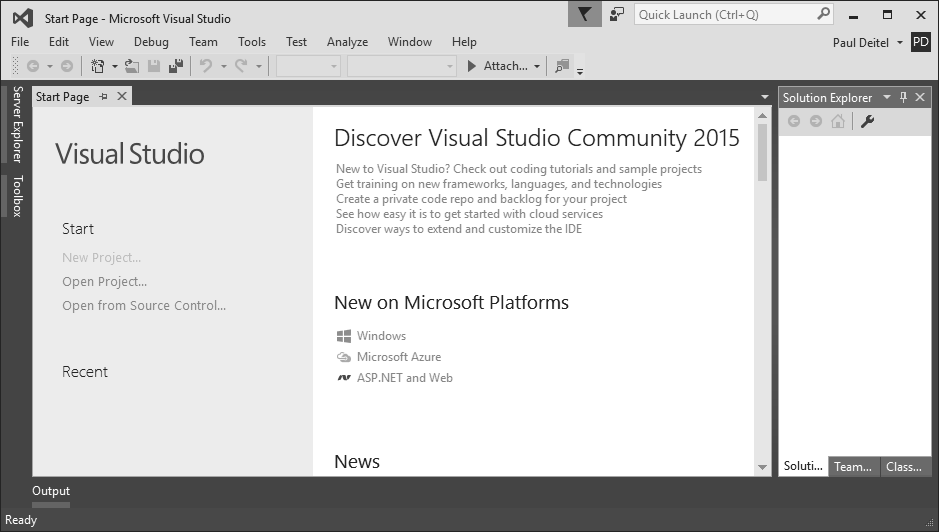
\includegraphics[width=0.95\textwidth,height=0.60\textheight,keepaspectratio]{images/fig2_01_start_page.png}\\
      \scriptsize \textbf{Hình 2.1:} Màn hình Start Page trong Visual Studio (Giáo trình Deitel, trang 3).
    \end{column}
  \end{columns}
\end{frame}

% ==============================================================================
% SLIDE 9: HỘP THOẠI TẠO DỰ ÁN MỚI (NEW PROJECT DIALOG)
% ==============================================================================
\begin{frame}{Hộp thoại Tạo Dự án Mới (New Project Dialog)}
  \begin{columns}[T]
    \begin{column}{0.45\textwidth}
      \textbf{Quy trình 4 bước tạo dự án chuẩn:}
      \begin{enumerate}\small
        \item \textbf{Chọn Ngôn ngữ:} Chọn \textbf{Visual C\#} ở ngăn phân cấp bên trái.
        \item \textbf{Chọn Mẫu ứng dụng:} Chọn \textbf{Windows Forms Application} ở ngăn giữa.
        \item \textbf{Đặt Tên dự án (Name):} Đặt tên gợi nhớ theo chuẩn PascalCase (ví dụ: \texttt{ASimpleApp}).
        \item \textbf{Chọn Thư mục lưu trữ (Location):} Trỏ đến thư mục bài tập của sinh viên (ví dụ: \texttt{D:\textbackslash CSharpLabs\textbackslash}).
      \end{enumerate}
      \begin{alertblock}{\textbf{Lưu ý quan trọng:}}
        Đánh dấu chọn \textit{"Create directory for solution"} để tạo thư mục Solution độc lập.
      \end{alertblock}
    \end{column}

    \begin{column}{0.53\textwidth}
      \centering
      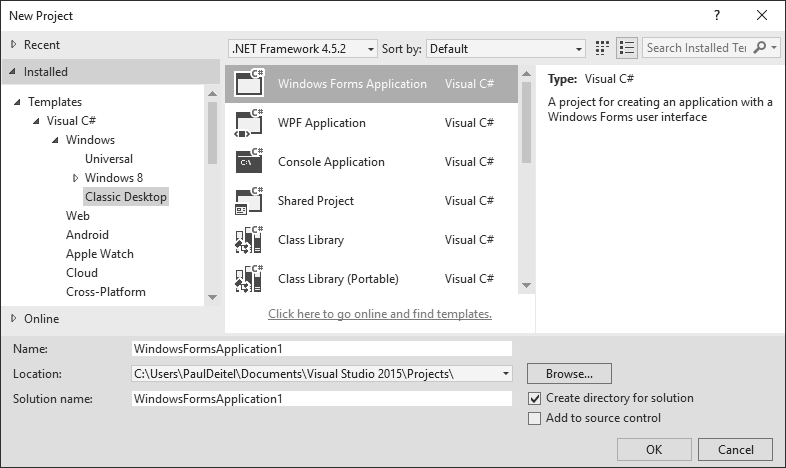
\includegraphics[width=0.95\textwidth,height=0.60\textheight,keepaspectratio]{images/fig2_03_new_project_dialog.png}\\
      \scriptsize \textbf{Hình 2.3:} Hộp thoại New Project dialog trong Visual Studio (Giáo trình Deitel, trang 5).
    \end{column}
  \end{columns}
\end{frame}

% ==============================================================================
% SLIDE 10: KHẢO SÁT GIAO DIỆN THIẾT KẾ DESIGN VIEW
% ==============================================================================
\begin{frame}{Khung nhìn Thiết kế Trực quan (Design View)}
  \begin{columns}[T]
    \begin{column}{0.45\textwidth}
      \textbf{Cấu trúc không gian làm việc IDE:}
      \begin{itemize}\small
        \item \textbf{Form Designer (ở giữa):} Vùng làm việc chính hiển thị biểu mẫu Form rỗng màu xám với tiêu đề mặc định \texttt{Form1}.
        \item \textbf{Toolbox (bên trái):} Chứa các điều khiển đồ họa sẵn sàng để kéo thả.
        \item \textbf{Solution Explorer (góc trên bên phải):} Quản lý cây tệp tin và cấu trúc dự án.
        \item \textbf{Properties Window (góc dưới bên phải):} Bảng thuộc tính của đối tượng đang chọn.
      \end{itemize}
    \end{column}

    \begin{column}{0.53\textwidth}
      \centering
      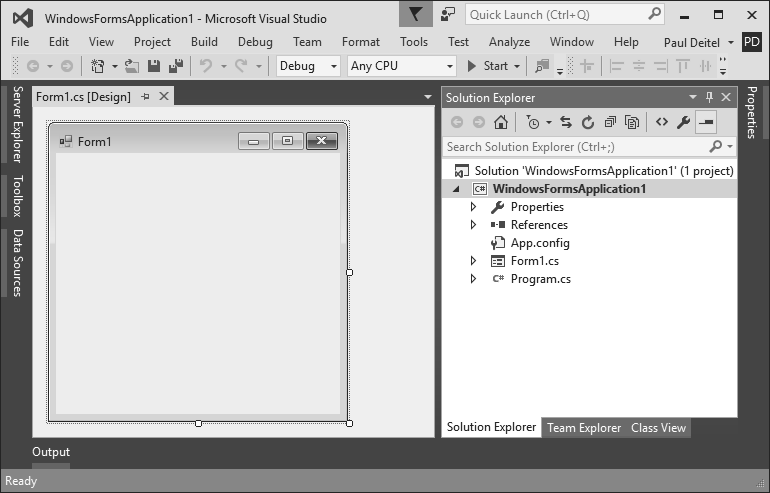
\includegraphics[width=0.95\textwidth,height=0.60\textheight,keepaspectratio]{images/fig2_04_design_view.png}\\
      \scriptsize \textbf{Hình 2.4:} Khung nhìn Design View khi mở dự án mới (Giáo trình Deitel, trang 6).
    \end{column}
  \end{columns}
\end{frame}

% ==============================================================================
% SLIDE 11: THANH MENU BAR - TỔNG QUAN CÁC THỰC ĐƠN
% ==============================================================================
\begin{frame}{Thanh Menu Bar -- Trung tâm Điều khiển Lệnh của IDE}
  \centering
  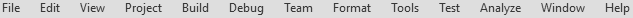
\includegraphics[width=0.95\textwidth,height=0.60\textheight,keepaspectratio]{images/fig2_05_menu_bar.png}\\[1mm]
  \scriptsize \textbf{Hình 2.5:} Thanh Menu Bar trong Visual Studio (Giáo trình Deitel, trang 7).\\[3mm]

  \begin{table}\footnotesize
    \centering
    \begin{tabularx}{\textwidth}{lXlX}
      \toprule
      \textbf{Menu} & \textbf{Chức năng cốt lõi} & \textbf{Menu} & \textbf{Chức năng cốt lõi} \\
      \midrule
      \textbf{File} & Tạo, mở, lưu, đóng tệp và dự án & \textbf{Debug} & Khởi chạy (F5), gỡ lỗi, Step Over (F10) \\
      \textbf{Edit} & Cut, Copy, Paste, Undo, Find \& Replace & \textbf{Format} & Căn hàng, dàn đều khoảng cách điều khiển \\
      \textbf{View} & Bật/tắt các cửa sổ (Toolbox, Properties) & \textbf{Tools} & Tùy biến cài đặt IDE, kết nối CSDL \\
      \textbf{Project} & Thêm Form mới, Class mới, Add Reference & \textbf{Window} & Bố trí cửa sổ (Split, Tabbed, Float) \\
      \textbf{Build} & Biên dịch dự án (Build Solution / Rebuild) & \textbf{Help} & Tra cứu tài liệu, mẫu mã, phím F1 \\
      \bottomrule
    \end{tabularx}
  \end{table}
\end{frame}

% ==============================================================================
% SLIDE 12: CHI TIẾT CÁC MENU QUAN TRỌNG: BUILD, DEBUG & FORMAT
% ==============================================================================
\begin{frame}{Chi tiết các Menu Quan trọng: Build, Debug \& Format}
  \begin{columns}[T]
    \begin{column}{0.32\textwidth}
      \begin{block}{\textbf{Menu BUILD}}
        \begin{itemize}\footnotesize
          \item \textbf{Build Solution (Ctrl+Shift+B):} Biên dịch toàn bộ các tệp mã nguồn trong giải pháp ra tệp \texttt{.exe} hoặc \texttt{.dll}.
          \item \textbf{Rebuild Solution:} Xóa sạch kết quả cũ và biên dịch lại từ đầu mọi tệp tin.
          \item \textbf{Clean Solution:} Xóa các tệp trung gian trong thư mục \texttt{bin/} và \texttt{obj/}.
        \end{itemize}
      \end{block}
    \end{column}

    \begin{column}{0.32\textwidth}
      \begin{block}{\textbf{Menu DEBUG}}
        \begin{itemize}\footnotesize
          \item \textbf{Start Debugging (F5):} Chạy ứng dụng có gắn trình gỡ lỗi (bắt lỗi Runtime).
          \item \textbf{Start Without Debugging (Ctrl+F5):} Chạy ứng dụng độc lập với tốc độ tối đa.
          \item \textbf{Toggle Breakpoint (F9):} Đặt điểm dừng trên dòng lệnh để kiểm tra biến.
        \end{itemize}
      \end{block}
    \end{column}

    \begin{column}{0.32\textwidth}
      \begin{exampleblock}{\textbf{Menu FORMAT}}
        \begin{itemize}\footnotesize
          \item Chỉ xuất hiện khi Form đang ở \textbf{Design View}.
          \item \textbf{Align:} Căn bằng mép trái, phải, trên, dưới giữa các điều khiển.
          \item \textbf{Make Same Size:} Đồng bộ kích thước Width/Height tự động.
          \item \textbf{Center in Form:} Căn chính giữa Form theo chiều ngang/dọc.
        \end{itemize}
      \end{exampleblock}
    \end{column}
  \end{columns}
\end{frame}

% ==============================================================================
% SLIDE 13: THANH CÔNG CỤ CHUẨN (STANDARD TOOLBAR)
% ==============================================================================
\begin{frame}{Thanh Công cụ Chuẩn (Standard Toolbar)}
  \begin{columns}[T]
    \begin{column}{0.45\textwidth}
      \textbf{Các nút bấm thao tác nhanh:}
      \begin{itemize}\small
        \item \textbf{New Project / Open File:} Phím tắt mở nhanh.
        \item \textbf{Save (Ctrl+S) / Save All (Ctrl+Shift+S):} Lưu tệp hiện tại hoặc lưu toàn bộ giải pháp.
        \item \textbf{Undo (Ctrl+Z) / Redo (Ctrl+Y):} Hoàn tác hoặc làm lại thao tác thiết kế.
        \item \textbf{Start Button (F5):} Nút mũi tên màu xanh lá để kích hoạt biên dịch và chạy thử.
        \item \textbf{Solution Configurations:} Chuyển đổi giữa chế độ \texttt{Debug} (gỡ lỗi) và \texttt{Release} (đóng gói phát hành).
      \end{itemize}
    \end{column}

    \begin{column}{0.53\textwidth}
      \centering
      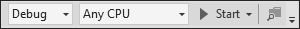
\includegraphics[width=0.95\textwidth,height=0.60\textheight,keepaspectratio]{images/fig2_07_standard_toolbar.png}\\[2mm]
      \scriptsize \textbf{Hình 2.7:} Thanh Standard Toolbar trong Visual Studio (Deitel, trang 8).\\[3mm]
      \begin{tcolorbox}[colback=UniLightBlue!30,colframe=UniBlue,title=\textbf{Mẹo tăng tốc:},fonttitle=\small\bfseries]
        \footnotesize Luôn duy trì thói quen nhấn \textbf{Ctrl+Shift+S} (Save All) trước khi chạy thử ứng dụng!
      \end{tcolorbox}
    \end{column}
  \end{columns}
\end{frame}

% ==============================================================================
% SLIDE 14: TÍNH NĂNG TOOLTIPS & PHÍM TẮT THƯỜNG DÙNG
% ==============================================================================
\begin{frame}{Tính năng Tooltips \& Bảng Phím tắt Thường dùng}
  \begin{columns}[T]
    \begin{column}{0.48\textwidth}
      \begin{block}{\textbf{Tooltips (Chú giải công cụ)}}
        \begin{itemize}\small
          \item Khi rê chuột qua bất kỳ nút bấm nào trên thanh công cụ, một hộp thoại văn bản nhỏ sẽ nổi lên.
          \item Cung cấp: \textbf{Tên chức năng} kèm theo \textbf{Tổ hợp phím tắt tương ứng}.
        \end{itemize}
      \end{block}
      \centering
      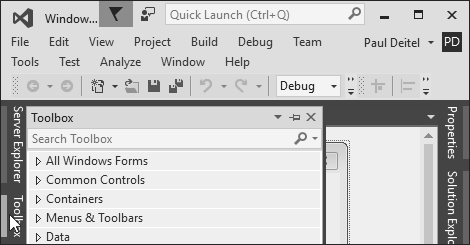
\includegraphics[width=0.95\textwidth,height=0.60\textheight,keepaspectratio]{images/fig2_11_hidden_toolbox.png}\\
      \scriptsize \textbf{Hình 2.11:} Hiển thị cửa sổ ẩn khi rê chuột.
    \end{column}

    \begin{column}{0.48\textwidth}
      \begin{exampleblock}{\textbf{Bảng Phím tắt Kỹ sư IT26M cần thuộc:}}
        \begin{table}\footnotesize
          \centering
          \begin{tabular}{ll}
            \toprule
            \textbf{Phím tắt} & \textbf{Hành động tương ứng} \\
            \midrule
            \textbf{F5} & Start Debugging (Chạy có gỡ lỗi) \\
            \textbf{Ctrl + F5} & Start Without Debugging (Chạy nhanh) \\
            \textbf{Shift + F5} & Dừng chương trình đang chạy \\
            \textbf{F4} & Bật cửa sổ Properties Window \\
            \textbf{Ctrl + Alt + X} & Bật cửa sổ Toolbox \\
            \textbf{Ctrl + Alt + L} & Bật cửa sổ Solution Explorer \\
            \textbf{F7 / Shift + F7} & Chuyển đổi giữa Code View \& Designer \\
            \textbf{Ctrl + Shift + B} & Biên dịch dự án (Build Solution) \\
            \bottomrule
          \end{tabular}
        \end{table}
      \end{exampleblock}
    \end{column}
  \end{columns}
\end{frame}

% ==============================================================================
% SLIDE 15: HỆ THỐNG TRỢ GIÚP THEO NGỮ CẢNH (CONTEXT-SENSITIVE HELP)
% ==============================================================================
\begin{frame}{Hệ thống Trợ giúp Ngữ cảnh (Context-Sensitive Help) \& Phím F1}
  \begin{columns}[T]
    \begin{column}{0.5\textwidth}
      \begin{block}{\textbf{Sức mạnh của phím F1:}}
        \begin{itemize}\small
          \item Khi đang chọn bất kỳ điều khiển GUI nào (ví dụ: Button, PictureBox) hoặc một từ khóa C\# trong Code Editor:
          \item \textbf{Nhấn phím F1:} Visual Studio sẽ tự động kích hoạt trình duyệt và điều hướng trực tiếp tới trang tài liệu chính thức của thành phần đó trên \textbf{Microsoft Learn / MSDN Library}.
          \item Sinh viên không cần tốn công gõ tìm kiếm thủ công trên Google.
        \end{itemize}
      \end{block}
      \begin{tcolorbox}[colback=UniOrange!10,colframe=UniOrange,title=\textbf{Văn hóa đọc tài liệu:},fonttitle=\small\bfseries]
        \footnotesize Kỹ sư phần mềm xuất sắc là người biết cách khai thác tài liệu chuẩn Microsoft để tự học thuộc tính và sự kiện mới!
      \end{tcolorbox}
    \end{column}

    \begin{column}{0.48\textwidth}
      \centering
      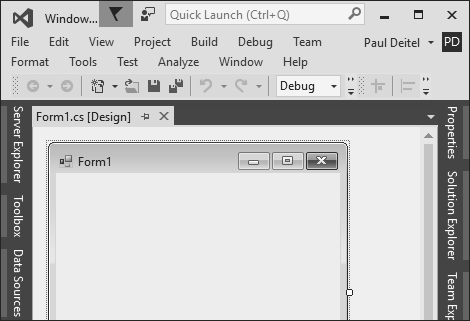
\includegraphics[width=0.95\textwidth,height=0.60\textheight,keepaspectratio]{images/fig2_10_autohide.png}\\
      \scriptsize \textbf{Hình 2.10:} Cơ chế tương tác trực quan với các thành phần IDE.
    \end{column}
  \end{columns}
\end{frame}

% ==============================================================================
% SLIDE 16: CHECKPOINT 1 - KIỂM TRA NHANH TIẾT 1
% ==============================================================================
\begin{frame}{Checkpoint 1: Kiểm tra Kiến thức Nhanh Tiết 1}
  \begin{alertblock}{\textbf{Câu hỏi 1:}}
    Tổ hợp phím tắt nào trong Visual Studio cho phép lập trình viên chạy ứng dụng ở chế độ độc lập với tốc độ cao nhất (không gắn trình gỡ lỗi Debugger)?
    \begin{enumerate}[(A)]
      \item Phím \textbf{F5}
      \item Tổ hợp phím \textbf{Ctrl + F5}
      \item Tổ hợp phím \textbf{Ctrl + Shift + B}
      \item Phím \textbf{F4}
    \end{enumerate}
  \end{alertblock}
  \pause
  \begin{exampleblock}{\textbf{Giải thích đáp án:}}
    \textbf{Đáp án chính xác: B (Ctrl + F5).} Phím F5 kích hoạt \textit{Start Debugging} (chạy có gỡ lỗi, kiểm tra bộ nhớ), trong khi \textbf{Ctrl + F5} là \textit{Start Without Debugging} giúp ứng dụng khởi chạy độc lập tức thì.
  \end{exampleblock}
\end{frame}

% ==============================================================================
% SLIDE 17: HANDS-ON LAB 1 - TẠO DỰ ÁN ĐẦU TAY
% ==============================================================================
\begin{frame}{Hands-on Lab 1: Khởi tạo Solution \& Khảo sát Menus (15 Phút)}
  \begin{columns}[T]
    \begin{column}{0.48\textwidth}
      \begin{tcolorbox}[colback=UniGreen!5,colframe=UniGreen,title=\textbf{NHIỆM VỤ THỰC HÀNH TẠI PHÒNG MÁY:},fonttitle=\small\bfseries]
        \begin{enumerate}\small
          \item Khởi động Visual Studio Community trên máy tính phòng máy.
          \item Chọn \textbf{File $\to$ New $\to$ Project...} (hoặc Ctrl+Shift+N).
          \item Chọn ngôn ngữ \textbf{Visual C\#} $\to$ \textbf{Windows Forms Application}.
          \item Đặt tên dự án: \texttt{Lab01\_VisualIntro\_IT26M}.
          \item Lưu vào thư mục cá nhân: \texttt{D:\textbackslash IT26M\_Labs\textbackslash}.
          \item Khảo sát thanh Menu Bar và Standard Toolbar.
          \item Nhấn \textbf{Ctrl + F5} để chạy thử biểu mẫu Form rỗng đầu tiên.
        \end{enumerate}
      \end{tcolorbox}
    \end{column}

    \begin{column}{0.48\textwidth}
      \begin{tcolorbox}[colback=UniNavy!5,colframe=UniNavy,title=\textbf{KẾT QUẢ MONG ĐỢI:},fonttitle=\small\bfseries]
        \begin{itemize}\small
          \item Cửa sổ Form1 màu xám xuất hiện ở giữa màn hình.
          \item Có đầy đủ 3 nút tiêu chuẩn trên thanh tiêu đề: Minimize, Maximize và Close (\texttt{X}).
          \item Kéo giãn cửa sổ bằng chuột để xác nhận Form hoạt động bình thường.
          \item Đóng cửa sổ để quay lại không gian thiết kế của Visual Studio.
        \end{itemize}
      \end{tcolorbox}
    \end{column}
  \end{columns}
\end{frame}

% ==============================================================================
% SLIDE 18: TIẾT 2 DIVIDER
% ==============================================================================
\begin{frame}[plain]
  \vfill
  \centering
  \begin{beamercolorbox}[sep=8pt,center,shadow=true,rounded=true]{palette secondary}
    {\Huge \textbf{TIẾT 2}}\\[2mm]
    {\Large \textbf{ĐIỀU HƯỚNG CỬA SỔ IDE, SOLUTION EXPLORER, TOOLBOX \& PROPERTIES}}
  \end{beamercolorbox}
  \vfill
\end{frame}

% ==============================================================================
% SLIDE 19: TÍNH NĂNG TỰ ĐỘNG ẨN CỬA SỔ (AUTO-HIDE & PINNING)
% ==============================================================================
\begin{frame}{Kỹ thuật Điều hướng: Tính năng Auto-Hide \& Nút Ghim (Pin Icon)}
  \begin{columns}[T]
    \begin{column}{0.48\textwidth}
      \begin{block}{\textbf{Cơ chế Tự động Ẩn (Auto-Hide):}}
        \begin{itemize}\small
          \item Khi không gian màn hình chật hẹp, ta có thể thu nhỏ các cửa sổ công cụ thành các tab chữ dọc mép màn hình.
          \item Khi rê chuột lên tab (ví dụ: \texttt{Toolbox}), cửa sổ sẽ trượt ra nhẹ nhàng để ta chọn điều khiển.
          \item Khi đưa chuột ra ngoài, cửa sổ tự động ẩn lại để giải phóng không gian cho Form Designer.
        \end{itemize}
      \end{block}

      \begin{exampleblock}{\textbf{Nút Ghim (Pin Icon):}}
        \begin{itemize}\small
          \item \textbf{Cây ghim nằm ngang:} Cửa sổ đang ở chế độ \textit{Auto-Hide}.
          \item \textbf{Cây ghim thẳng đứng:} Cửa sổ được \textit{"ghim chặt"} cố định trên màn hình làm việc.
        \end{itemize}
      \end{exampleblock}
    \end{column}

    \begin{column}{0.48\textwidth}
      \centering
      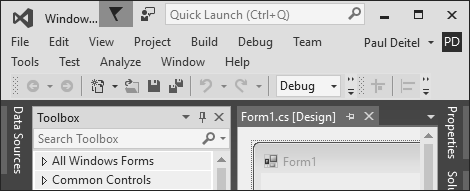
\includegraphics[width=0.95\textwidth,height=0.60\textheight,keepaspectratio]{images/fig2_12_pinning_window.png}\\[2mm]
      \scriptsize \textbf{Hình 2.12:} Nút cây ghim (Pin icon) để tắt tính năng Auto-Hide (Deitel, trang 11).
    \end{column}
  \end{columns}
\end{frame}

% ==============================================================================
% SLIDE 20: KỸ THUẬT DOCKING, TÁCH TAB & BỐ TRÍ CỬA SỔ
% ==============================================================================
\begin{frame}{Kỹ thuật Ghép nối Cửa sổ (Docking \& Tab Groups)}
  \begin{columns}[T]
    \begin{column}{0.5\textwidth}
      \begin{block}{\textbf{Kỹ thuật Docking chuyên nghiệp:}}
        \begin{itemize}\small
          \item Kéo thanh tiêu đề của bất kỳ cửa sổ nào, Visual Studio sẽ hiển thị \textbf{Bánh dẫn đường Docking Guide} hình chữ thập.
          \item Kéo chuột vào mũi tên:
            \begin{itemize}\footnotesize
              \item \textbf{Top / Bottom / Left / Right:} Chia đôi không gian màn hình theo hướng tương ứng.
              \item \textbf{Center:} Nhập cửa sổ thành một tab chung với cửa sổ hiện có.
            \end{itemize}
        \end{itemize}
      \end{block}
      \begin{tcolorbox}[colback=UniLightBlue!30,colframe=UniBlue,title=\textbf{Khôi phục bố cục mặc định:},fonttitle=\small\bfseries]
        \footnotesize Nếu lỡ tay làm lộn xộn cửa sổ, chỉ cần vào: \textbf{Window $\to$ Reset Window Layout} để trở về trạng thái chuẩn ban đầu!
      \end{tcolorbox}
    \end{column}

    \begin{column}{0.48\textwidth}
      \begin{tcolorbox}[colback=CSharpPurple!10,colframe=CSharpPurple,title=\textbf{3 Trạng thái Hiển thị Cửa sổ:},fonttitle=\small\bfseries]
        \begin{enumerate}\small
          \item \textbf{Docked (Neo cố định):} Gắn chặt vào một mép của khung nhìn IDE.
          \item \textbf{Floating (Trôi nổi tự do):} Kéo rời ra ngoài thành một cửa sổ Windows độc lập (tiện lợi khi dùng 2 màn hình).
          \item \textbf{Tabbed Document (Thẻ văn bản):} Xếp chồng thành các tab tài liệu (Form1.cs, Form1.Designer.cs).
        \end{enumerate}
      \end{tcolorbox}
    \end{column}
  \end{columns}
\end{frame}

% ==============================================================================
% SLIDE 21: CỬA SỔ SOLUTION EXPLORER - CẤU TRÚC PHÂN CẤP
% ==============================================================================
\begin{frame}{Cửa sổ Solution Explorer: Cấu trúc Giải pháp \& Dự án}
  \begin{columns}[T]
    \begin{column}{0.48\textwidth}
      \begin{block}{\textbf{Phân cấp Solution \& Project:}}
        \begin{itemize}\small
          \item \textbf{Solution (Tệp \texttt{.sln}):} Container cấp cao nhất, có thể quản lý một hoặc nhiều dự án liên quan cùng các thiết lập biên dịch chung.
          \item \textbf{Project (Tệp \texttt{.csproj}):} Đơn vị cấu thành phần mềm, chứa các tệp mã nguồn C\#, tài nguyên hình ảnh, biểu tượng và cấu hình dependencies.
          \item Cho phép kích chuột phải để thêm tệp mới, đổi tên hoặc thiết lập dự án khởi động (\textit{Set as Startup Project}).
        \end{itemize}
      \end{block}
    \end{column}

    \begin{column}{0.48\textwidth}
      \centering
      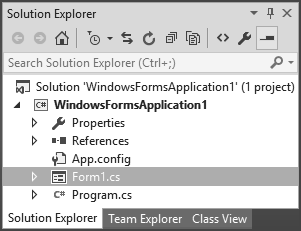
\includegraphics[width=0.95\textwidth,height=0.60\textheight,keepaspectratio]{images/fig2_13_solution_explorer.png}\\[1mm]
      \scriptsize \textbf{Hình 2.13:} Cửa sổ Solution Explorer (Giáo trình Deitel, trang 11).
    \end{column}
  \end{columns}
\end{frame}

% ==============================================================================
% SLIDE 22: CHI TIẾT CÁC TỆP TIN TRONG MỘT DỰ ÁN WINFORMS
% ==============================================================================
\begin{frame}{Giải phẫu các Tệp tin trong Dự án Windows Forms}
  \begin{table}\footnotesize
    \centering
    \begin{tabularx}{\textwidth}{lX}
      \toprule
      \textbf{Tên Tệp Tin / Nút} & \textbf{Ý nghĩa Kỹ thuật \& Vai trò} \\
      \midrule
      \textbf{Solution (.sln)} & Tệp văn bản quản lý danh sách các Project và cấu hình build (Debug/Release). \\
      \textbf{Project (.csproj)} & Tệp XML đặc tả các tệp mã nguồn, phiên bản .NET SDK và các gói thư viện NuGet. \\
      \textbf{Properties / App.config} & Chứa thông tin bản quyền ứng dụng, chuỗi kết nối cơ sở dữ liệu và cài đặt cấu hình. \\
      \textbf{References} & Danh sách các thư viện liên kết động (.dll) của .NET Framework mà dự án sử dụng. \\
      \textbf{Form1.cs} & Tệp mã nguồn C\# chứa logic ứng dụng và các hàm xử lý sự kiện (Event Handlers) do lập trình viên viết. \\
      \textbf{Form1.Designer.cs} & Tệp C\# do Visual Studio tự động sinh ra và cập nhật mỗi khi lập trình viên kéo-thả điều khiển trên Form. \\
      \textbf{Form1.resx} & Tệp tài nguyên XML lưu trữ hình ảnh, chuỗi đa ngôn ngữ nhúng bên trong Form. \\
      \textbf{Program.cs} & Tệp chứa điểm vào (Entry Point) của ứng dụng -- hàm \texttt{static void Main()} khởi chạy Form. \\
      \bottomrule
    \end{tabularx}
  \end{table}
  \vspace{-1mm}
  \begin{alertblock}{\textbf{Cảnh báo vàng:}}
    Sinh viên tuyệt đối \textbf{không sửa tay trực tiếp} nội dung bên trong tệp \texttt{Form1.Designer.cs} trừ khi thực sự hiểu rõ, vì IDE có thể ghi đè làm hỏng giao diện Form Designer!
  \end{alertblock}
\end{frame}

% ==============================================================================
% SLIDE 23: NÚT REFERENCES - QUẢN LÝ THƯ VIỆN LIÊN KẾT
% ==============================================================================
\begin{frame}{Nút References -- Quản lý Thư viện Liên kết (Assemblies)}
  \begin{columns}[T]
    \begin{column}{0.48\textwidth}
      \begin{block}{\textbf{Vai trò của nút References:}}
        \begin{itemize}\small
          \item Một ứng dụng C\# không thể chạy độc lập nếu thiếu các thư viện lớp cơ sở của .NET (Framework Class Library).
          \item Nút \textbf{References} hiển thị tất cả các Assembly (.dll) được nạp vào dự án:
            \begin{itemize}\footnotesize
              \item \texttt{System}: Các kiểu dữ liệu cơ bản, ngoại lệ, I/O.
              \item \texttt{System.Drawing}: Xử lý đồ họa, màu sắc, font chữ.
              \item \texttt{System.Windows.Forms}: Chứa các lớp điều khiển GUI (Form, Button, TextBox...).
            \end{itemize}
        \end{itemize}
      \end{block}
    \end{column}

    \begin{column}{0.48\textwidth}
      \centering
      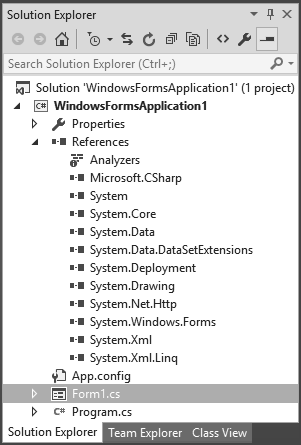
\includegraphics[width=0.95\textwidth,height=0.60\textheight,keepaspectratio]{images/fig2_14_solution_explorer_references.png}\\[1mm]
      \scriptsize \textbf{Hình 2.14:} Cây References được mở rộng (Giáo trình Deitel, trang 12).
    \end{column}
  \end{columns}
\end{frame}

% ==============================================================================
% SLIDE 24: CỬA SỔ TOOLBOX - KHO LINH KIỆN ĐỒ HỌA
% ==============================================================================
\begin{frame}{Cửa sổ Toolbox -- Kho Linh kiện Điều khiển Đồ họa}
  \begin{columns}[T]
    \begin{column}{0.5\textwidth}
      \begin{block}{\textbf{Cấu trúc phân loại trong Toolbox:}}
        \begin{itemize}\small
          \item Chứa tất cả các điều khiển giao diện (Controls) có thể đưa lên Form.
          \item Phân chia thành các nhóm chủ đề có thể thu gọn/mở rộng:
            \begin{itemize}\footnotesize
              \item \textbf{Common Controls:} Các điều khiển phổ biến nhất (Button, Label, TextBox, CheckBox, RadioButton, PictureBox...).
              \item \textbf{Containers:} Khung chứa phân nhóm điều khiển (GroupBox, Panel, TabControl...).
              \item \textbf{Menus \& Toolbars:} Tạo hệ thống menu thả và thanh công cụ.
              \item \textbf{Data:} Điều khiển hiển thị dữ liệu lưới (DataGridView).
            \end{itemize}
        \end{itemize}
      \end{block}
    \end{column}

    \begin{column}{0.48\textwidth}
      \begin{exampleblock}{\textbf{2 Cách đưa điều khiển lên Form:}}
        \begin{enumerate}\small
          \item \textbf{Cách 1 (Kéo-Thả):} Nhấn giữ chuột trái vào điều khiển trong Toolbox, kéo rê vào Form rồi thả ra tại vị trí mong muốn.
          \item \textbf{Cách 2 (Nhấp đúp chuột):} Nhấp đúp chuột trái vào biểu tượng điều khiển trong Toolbox, điều khiển sẽ tự động xuất hiện ở góc trên bên trái của Form.
        \end{enumerate}
      \end{exampleblock}
    \end{column}
  \end{columns}
\end{frame}

% ==============================================================================
% SLIDE 25: KHÁM PHÁ NHÓM COMMON CONTROLS
% ==============================================================================
\begin{frame}{Khám phá Nhóm Common Controls Thông dụng}
  \begin{columns}[T]
    \begin{column}{0.48\textwidth}
      \centering
      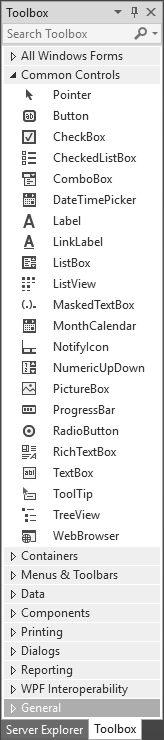
\includegraphics[width=0.95\textwidth,height=0.60\textheight,keepaspectratio]{images/fig2_15_toolbox_common_controls.png}\\[1mm]
      \scriptsize \textbf{Hình 2.15:} Nhóm Common Controls trong Toolbox (Deitel, trang 13).
    \end{column}

    \begin{column}{0.5\textwidth}
      \begin{table}\footnotesize
        \centering
        \begin{tabularx}{\textwidth}{lX}
          \toprule
          \textbf{Điều khiển} & \textbf{Công dụng trực quan chính} \\
          \midrule
          \textbf{Label} & Hiển thị nhãn văn bản cố định, hướng dẫn người dùng. \\
          \textbf{TextBox} & Hộp cho phép người dùng nhập dữ liệu văn bản từ bàn phím. \\
          \textbf{Button} & Nút bấm kích hoạt hành động khi người dùng nhấp chuột. \\
          \textbf{PictureBox} & Khung chuyên dụng hiển thị hình ảnh đồ họa (BMP, JPG, PNG). \\
          \textbf{CheckBox} & Nút chọn nhiều mục độc lập (Bật / Tắt trạng thái). \\
          \textbf{RadioButton} & Nút chọn tròn độc quyền (chỉ chọn 1 trong nhóm). \\
          \bottomrule
        \end{tabularx}
      \end{table}
    \end{column}
  \end{columns}
\end{frame}

% ==============================================================================
% SLIDE 26: CỬA SỔ PROPERTIES WINDOW - CẤU HÌNH THỜI ĐIỂM THIẾT KẾ
% ==============================================================================
\begin{frame}{Cửa sổ Properties Window: Cấu hình Lúc Thiết kế (Design-Time)}
  \begin{columns}[T]
    \begin{column}{0.48\textwidth}
      \begin{block}{\textbf{Cấu trúc của Properties Window:}}
        \begin{itemize}\small
          \item \textbf{Object Dropdown List (ở trên cùng):} Hiển thị tên định danh và kiểu của điều khiển đang được chọn (ví dụ: \texttt{Form1 System.Windows.Forms.Form}).
          \item \textbf{Thanh công cụ chuyển chế độ xem:}
            \begin{itemize}\footnotesize
              \item Categorized (phân nhóm) vs Alphabetical (A-Z).
              \item Properties (thuộc tính) vs Events (sự kiện - biểu tượng tia sét).
            \end{itemize}
          \item \textbf{Bảng 2 cột:} Cột trái là \textbf{Tên thuộc tính}, cột phải là \textbf{Giá trị thiết lập}.
          \item \textbf{Description Pane (ở đáy):} Tóm tắt ngắn gọn ý nghĩa của thuộc tính đang chọn.
        \end{itemize}
      \end{block}
    \end{column}

    \begin{column}{0.48\textwidth}
      \centering
      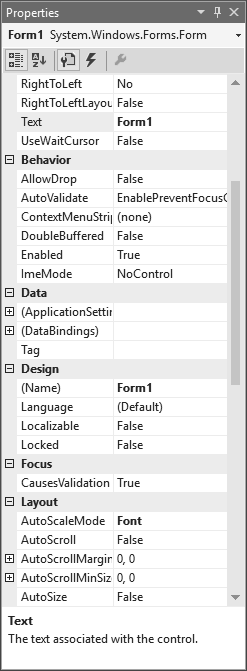
\includegraphics[width=0.95\textwidth,height=0.60\textheight,keepaspectratio]{images/fig2_16_properties_window.png}\\[1mm]
      \scriptsize \textbf{Hình 2.16:} Cửa sổ Properties Window của Form1 (Deitel, trang 14).
    \end{column}
  \end{columns}
\end{frame}

% ==============================================================================
% SLIDE 27: HAI CHẾ ĐỘ XEM PROPERTIES: ALPHABETICAL VS CATEGORIZED
% ==============================================================================
\begin{frame}{Hai Chế độ Xem Properties: Alphabetical vs Categorized}
  \begin{columns}[T]
    \begin{column}{0.48\textwidth}
      \begin{block}{\textbf{Chế độ Categorized (Phân nhóm theo chủ đề)}}
        \begin{itemize}\small
          \item Gom nhóm các thuộc tính có cùng tính chất kỹ thuật:
            \begin{itemize}\footnotesize
              \item \textbf{Appearance:} BackColor, Font, ForeColor, Text.
              \item \textbf{Behavior:} Enabled, Visible.
              \item \textbf{Design:} (Name) -- Tên biến định danh điều khiển.
              \item \textbf{Layout:} Location, Size, AutoSize, Dock, Anchor.
            \end{itemize}
          \item Thích hợp cho người mới bắt đầu làm quen để hiểu phân loại.
        \end{itemize}
      \end{block}
    \end{column}

    \begin{column}{0.48\textwidth}
      \begin{exampleblock}{\textbf{Chế độ Alphabetical (Sắp xếp A $\to$ Z)}}
        \begin{itemize}\small
          \item Xếp toàn bộ danh sách thuộc tính theo thứ tự bảng chữ cái từ A đến Z (ngoại trừ thuộc tính \texttt{(Name)} luôn đặt ở đầu).
          \item Được các kỹ sư phần mềm chuyên nghiệp ưa chuộng vì tìm kiếm cực nhanh khi đã biết rõ tên thuộc tính cần chỉnh (ví dụ: gõ chữ `T` để nhảy ngay đến `Text`).
        \end{itemize}
      \end{exampleblock}
    \end{column}
  \end{columns}
\end{frame}

% ==============================================================================
% SLIDE 28: CHECKPOINT 2 - KIỂM TRA NHANH TIẾT 2
% ==============================================================================
\begin{frame}{Checkpoint 2: Kiểm tra Kiến thức Nhanh Tiết 2}
  \begin{alertblock}{\textbf{Câu hỏi 2:}}
    Tệp tin nào sau đây chứa toàn bộ mã nguồn khởi tạo điều khiển đồ họa do Visual Studio tự động sinh ra khi lập trình viên thực hiện thao tác kéo-thả trên Form Designer?
    \begin{enumerate}[(A)]
      \item Tệp \texttt{Program.cs}
      \item Tệp \texttt{Form1.cs}
      \item Tệp \texttt{Form1.Designer.cs}
      \item Tệp cấu hình \texttt{App.config}
    \end{enumerate}
  \end{alertblock}
  \pause
  \begin{exampleblock}{\textbf{Giải thích đáp án:}}
    \textbf{Đáp án chính xác: C (\texttt{Form1.Designer.cs}).} Visual Studio áp dụng cơ chế lớp bộ phận (\texttt{partial class}) để tách biệt hoàn toàn mã giao diện tự sinh (\texttt{Form1.Designer.cs}) ra khỏi mã logic xử lý sự kiện của lập trình viên (\texttt{Form1.cs}).
  \end{exampleblock}
\end{frame}

% ==============================================================================
% SLIDE 29: HANDS-ON LAB 2 - TÙY BIẾN THUỘC TÍNH FORM
% ==============================================================================
\begin{frame}{Hands-on Lab 2: Sắp xếp Giao diện \& Tùy biến Form (15 Phút)}
  \begin{columns}[T]
    \begin{column}{0.48\textwidth}
      \begin{tcolorbox}[colback=CSharpPurple!5,colframe=CSharpPurple,title=\textbf{NHIỆM VỤ THỰC HÀNH TẠI CHỖ:},fonttitle=\small\bfseries]
        \begin{enumerate}\small
          \item Trên dự án \texttt{Lab01}, mở cửa sổ \textbf{Properties Window} (phím F4).
          \item Chuyển đổi qua lại giữa hai chế độ xem \textbf{Alphabetical} và \textbf{Categorized}.
          \item Tìm thuộc tính \textbf{Text} của Form, đổi giá trị từ \texttt{Form1} thành:
            \begin{center}\textbf{"Học phần Kỹ thuật Lập trình IT26M"}\end{center}
          \item Tìm thuộc tính \textbf{StartPosition}, chọn giá trị: \texttt{CenterScreen}.
          \item Bật tính năng \textbf{Auto-Hide} trên cửa sổ Toolbox, sau đó dùng nút ghim (Pin icon) để cố định lại.
        \end{enumerate}
      \end{tcolorbox}
    \end{column}

    \begin{column}{0.48\textwidth}
      \begin{tcolorbox}[colback=UniNavy!5,colframe=UniNavy,title=\textbf{KẾT QUẢ KIỂM CHỨNG:},fonttitle=\small\bfseries]
        \begin{itemize}\small
          \item Thanh tiêu đề của Form trên màn hình Design View lập tức đổi thành chuỗi tiếng Việt mới.
          \item Nhấn \textbf{Ctrl + F5}: Cửa sổ chương trình xuất hiện ngay chính giữa màn hình máy tính nhờ thuộc tính \texttt{CenterScreen}.
          \item Sinh viên làm chủ kỹ thuật ghim/thả các cửa sổ làm việc không bị lúng túng khi thao tác.
        \end{itemize}
      \end{tcolorbox}
    \end{column}
  \end{columns}
\end{frame}

% ==============================================================================
% SLIDE 30: TIẾT 3 DIVIDER
% ==============================================================================
\begin{frame}[plain]
  \vfill
  \centering
  \begin{beamercolorbox}[sep=8pt,center,shadow=true,rounded=true]{palette tertiary}
    {\Huge \textbf{TIẾT 3}}\\[2mm]
    {\Large \textbf{CASE STUDY THỰC HÀNH `ASimpleApp` (TEXT \& IMAGE) \& KIỂM THỬ}}
  \end{beamercolorbox}
  \vfill
\end{frame}

% ==============================================================================
% SLIDE 31: GIỚI THIỆU CASE STUDY ỨNG DỤNG `ASimpleApp`
% ==============================================================================
\begin{frame}{Giới thiệu Case Study: Xây dựng Ứng dụng `ASimpleApp`}
  \begin{columns}[T]
    \begin{column}{0.5\textwidth}
      \begin{block}{\textbf{Mục tiêu Case Study (Mục 2.6 SGK):}}
        \begin{itemize}\small
          \item Xây dựng một ứng dụng đồ họa Windows Forms hoàn chỉnh từ đầu mà \textbf{chưa cần viết một dòng mã C\# nào}.
          \item Rèn luyện kỹ năng sử dụng thành thạo:
            \begin{enumerate}\footnotesize
              \item Điều khiển \textbf{Form} (biểu mẫu nền, màu sắc, tiêu đề).
              \item Điều khiển \textbf{Label} (hiển thị văn bản chào mừng, tùy biến Font).
              \item Điều khiển \textbf{PictureBox} (hiển thị hình ảnh linh vật có co giãn).
            \end{enumerate}
        \end{itemize}
      \end{block}
    \end{column}

    \begin{column}{0.48\textwidth}
      \centering
      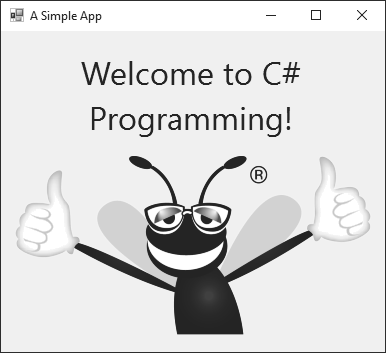
\includegraphics[width=0.95\textwidth,height=0.60\textheight,keepaspectratio]{images/fig2_17_simple_app_executing.png}\\[1mm]
      \scriptsize \textbf{Hình 2.17:} Mục tiêu thành phẩm: Ứng dụng ASimpleApp khi chạy (Deitel, trang 15).
    \end{column}
  \end{columns}
\end{frame}

% ==============================================================================
% SLIDE 32: BƯỚC 1: KHỞI TẠO DỰ ÁN `ASimpleApp`
% ==============================================================================
\begin{frame}{Bước 1: Khởi tạo Dự án `ASimpleApp` trong Visual Studio}
  \begin{columns}[T]
    \begin{column}{0.48\textwidth}
      \begin{enumerate}\small
        \item Mở Visual Studio, chọn \textbf{File $\to$ New $\to$ Project...}
        \item Chọn mẫu \textbf{Visual C\# $\to$ Windows Forms Application}.
        \item Tại ô \textbf{Name}: Nhập chính xác tên dự án là \texttt{ASimpleApp}.
        \item Tại ô \textbf{Location}: Trỏ vào thư mục bài tập của sinh viên.
        \item Nhấn nút \textbf{OK} để IDE tự động khởi tạo khung giải pháp mới.
      \end{enumerate}
    \end{column}

    \begin{column}{0.48\textwidth}
      \centering
      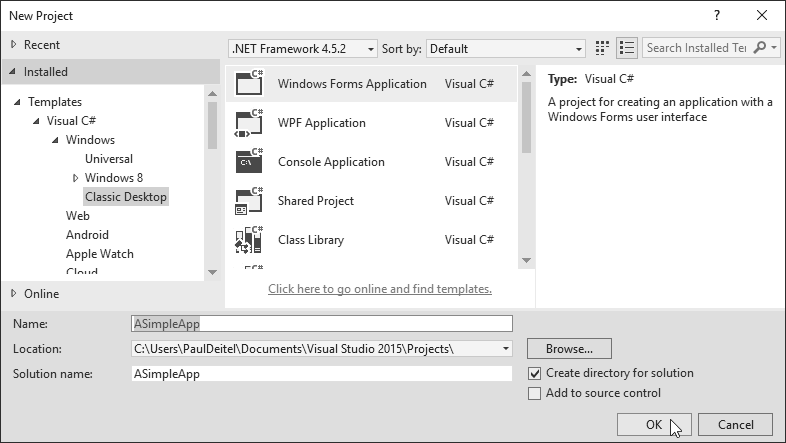
\includegraphics[width=0.95\textwidth,height=0.60\textheight,keepaspectratio]{images/fig2_18_new_project_asimpleapp.png}\\[1mm]
      \scriptsize \textbf{Hình 2.18:} Đặt tên dự án ASimpleApp trong New Project dialog (Deitel, trang 16).
    \end{column}
  \end{columns}
\end{frame}

% ==============================================================================
% SLIDE 33: BƯỚC 2: TÙY BIẾN THUỘC TÍNH FORM - TEXT & SIZING HANDLES
% ==============================================================================
\begin{frame}{Bước 2: Tùy biến Tiêu đề Form \& Kéo giãn Kích thước}
  \begin{columns}[T]
    \begin{column}{0.48\textwidth}
      \begin{block}{\textbf{Đổi Tiêu đề Form (Text Property):}}
        \begin{itemize}\small
          \item Chọn Form trên màn hình Design View.
          \item Trong cửa sổ Properties, tìm thuộc tính \textbf{Text}.
          \item Nhập giá trị mới: \textbf{\texttt{A Simple App}}.
          \item Tiêu đề trên thanh tiêu đề Form lập tức cập nhật.
        \end{itemize}
      \end{block}

      \begin{exampleblock}{\textbf{Điểm mút thay đổi kích thước (Sizing Handles):}}
        \begin{itemize}\small
          \item Quanh viền Form xuất hiện 8 chấm vuông nhỏ màu trắng gọi là \textit{sizing handles}.
          \item Rê chuột vào chấm góc dưới bên phải, con trỏ chuột chuyển thành mũi tên chéo hai đầu ($\searrow$).
          \item Kéo chuột để mở rộng kích thước Form.
        \end{itemize}
      \end{exampleblock}
    \end{column}

    \begin{column}{0.48\textwidth}
      \centering
      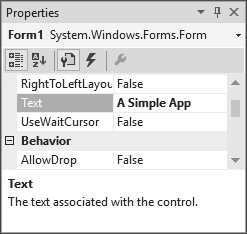
\includegraphics[width=0.85\textwidth,height=0.28\textheight,keepaspectratio]{images/fig2_19_form_text_property.png}\\[1mm]
      \scriptsize \textbf{Hình 2.19:} Đổi thuộc tính Text của Form (Deitel, trang 16).\\[2mm]
      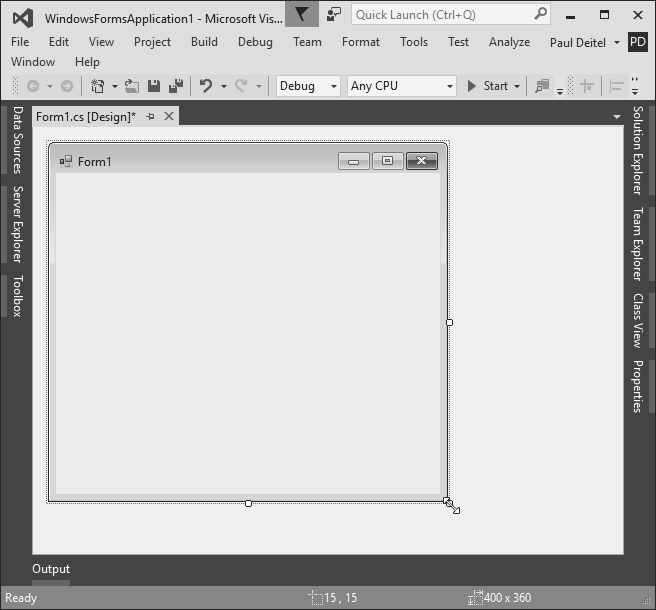
\includegraphics[width=0.85\textwidth,height=0.28\textheight,keepaspectratio]{images/fig2_21_resizing_form.png}\\[1mm]
      \scriptsize \textbf{Hình 2.21:} Thao tác kéo giãn Form qua sizing handle (Deitel, trang 17).
    \end{column}
  \end{columns}
\end{frame}

% ==============================================================================
% SLIDE 34: BƯỚC 3: TÙY BIẾN MÀU NỀN FORM (BACKCOLOR PROPERTY)
% ==============================================================================
\begin{frame}{Bước 3: Tùy biến Màu nền Form (BackColor Property)}
  \begin{columns}[T]
    \begin{column}{0.48\textwidth}
      \begin{block}{\textbf{Cấu hình thuộc tính BackColor:}}
        \begin{itemize}\small
          \item Tìm thuộc tính \textbf{BackColor} trong Properties Window.
          \item Nhấp vào mũi tên thả xuống ở cột giá trị để mở \textbf{Color Palette}:
            \begin{itemize}\footnotesize
              \item \textbf{Custom:} Chọn màu tùy ý theo mã RGB.
              \item \textbf{Web:} Bảng tên màu web chuẩn quốc tế.
              \item \textbf{System:} Màu theo chủ đề hệ điều hành Windows.
            \end{itemize}
          \item Chọn tab \textbf{Web} $\to$ chọn màu \textbf{LightCyan} (hoặc màu xanh nhạt).
        \end{itemize}
      \end{block}
    \end{column}

    \begin{column}{0.48\textwidth}
      \centering
      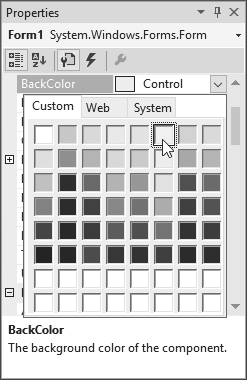
\includegraphics[width=0.85\textwidth,height=0.28\textheight,keepaspectratio]{images/fig2_22_form_backcolor.png}\\[1mm]
      \scriptsize \textbf{Hình 2.22:} Bảng chọn màu BackColor (Deitel, trang 18).\\[2mm]
      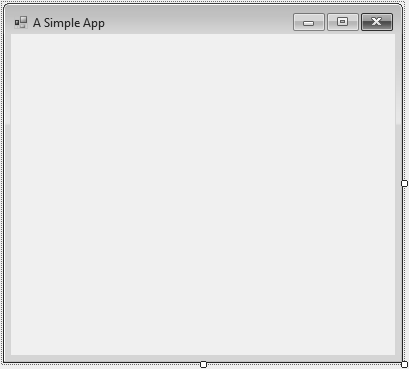
\includegraphics[width=0.85\textwidth,height=0.28\textheight,keepaspectratio]{images/fig2_23_form_new_backcolor.png}\\[1mm]
      \scriptsize \textbf{Hình 2.23:} Form sau khi nhận màu nền LightCyan (Deitel, trang 18).
    \end{column}
  \end{columns}
\end{frame}

% ==============================================================================
% SLIDE 35: BƯỚC 4: THÊM ĐIỀU KHIỂN LABEL & THIẾT LẬP NỘI DUNG
% ==============================================================================
\begin{frame}{Bước 4: Thêm Điều khiển Label \& Đổi Nội dung Văn bản}
  \begin{columns}[T]
    \begin{column}{0.48\textwidth}
      \begin{block}{\textbf{Thao tác thêm Label:}}
        \begin{itemize}\small
          \item Mở cửa sổ \textbf{Toolbox} $\to$ nhóm \textbf{Common Controls}.
          \item Kéo thả điều khiển \textbf{Label} vào vị trí phía trên cùng của Form.
          \item Điều khiển xuất hiện với tên mặc định là \texttt{label1}.
          \item Trong Properties Window, tìm thuộc tính \textbf{Text}.
          \item Nhập nội dung mới:
            \begin{center}\textbf{\texttt{Welcome to Visual C\#!}}\end{center}
        \end{itemize}
      \end{block}
    \end{column}

    \begin{column}{0.48\textwidth}
      \centering
      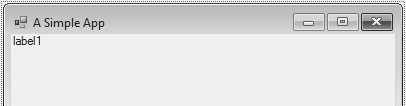
\includegraphics[width=0.85\textwidth,height=0.28\textheight,keepaspectratio]{images/fig2_24_adding_label.png}\\[1mm]
      \scriptsize \textbf{Hình 2.24:} Kéo thả Label từ Toolbox vào Form (Deitel, trang 19).\\[2mm]
      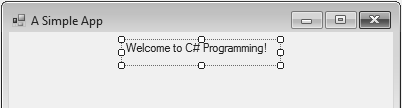
\includegraphics[width=0.85\textwidth,height=0.28\textheight,keepaspectratio]{images/fig2_25_gui_form_label.png}\\[1mm]
      \scriptsize \textbf{Hình 2.25:} Giao diện sau khi đổi chuỗi chào mừng (Deitel, trang 19).
    \end{column}
  \end{columns}
\end{frame}

% ==============================================================================
% SLIDE 36: BƯỚC 5: TÙY BIẾN FONT CHỮ QUA HỘP THOẠI FONT DIALOG
% ==============================================================================
\begin{frame}{Bước 5: Tùy biến Font Chữ qua Hộp thoại Font Dialog}
  \begin{columns}[T]
    \begin{column}{0.48\textwidth}
      \begin{block}{\textbf{Cấu hình thuộc tính Font của Label:}}
        \begin{itemize}\small
          \item Chọn điều khiển Label trên Form.
          \item Trong Properties Window, tìm thuộc tính \textbf{Font}.
          \item Nhấp vào nút có dấu ba chấm \textbf{\texttt{[...]}} ở bên phải giá trị để mở \textbf{Font Dialog}.
          \item Thiết lập các thông số:
            \begin{itemize}\footnotesize
              \item \textbf{Font:} \texttt{Segoe UI} (hoặc Tahoma).
              \item \textbf{Font style:} \textbf{Bold} (Đậm).
              \item \textbf{Size:} \textbf{24} points.
            \end{itemize}
          \item Nhấn \textbf{OK} để áp dụng font chữ lớn, sắc nét.
        \end{itemize}
      \end{block}
    \end{column}

    \begin{column}{0.48\textwidth}
      \centering
      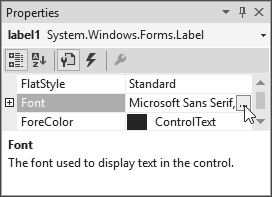
\includegraphics[width=0.85\textwidth,height=0.28\textheight,keepaspectratio]{images/fig2_26_label_font_property.png}\\[1mm]
      \scriptsize \textbf{Hình 2.26:} Nút mở rộng thuộc tính Font (Deitel, trang 20).\\[2mm]
      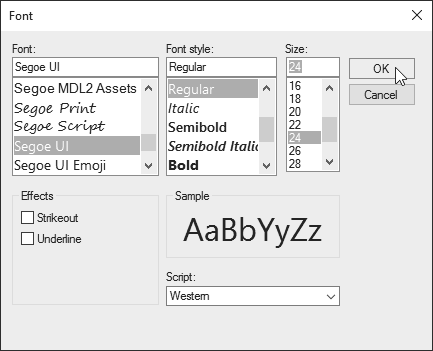
\includegraphics[width=0.85\textwidth,height=0.28\textheight,keepaspectratio]{images/fig2_27_font_dialog.png}\\[1mm]
      \scriptsize \textbf{Hình 2.27:} Hộp thoại Font dialog chuẩn (Deitel, trang 20).
    \end{column}
  \end{columns}
\end{frame}

% ==============================================================================
% SLIDE 37: BƯỚC 6: CĂN CHỈNH VĂN BẢN (TEXTALIGN PROPERTY)
% ==============================================================================
\begin{frame}{Bước 6: Căn giữa Văn bản với Thuộc tính TextAlign}
  \begin{columns}[T]
    \begin{column}{0.48\textwidth}
      \begin{block}{\textbf{Thiết lập Căn lề Hoàn hảo:}}
        \begin{itemize}\small
          \item Đặt thuộc tính \textbf{AutoSize} của Label thành \textbf{False} để cho phép tự do kéo giãn kích thước khung Label theo chiều ngang bằng Form.
          \item Tìm thuộc tính \textbf{TextAlign} trong Properties Window.
          \item Nhấp chuột vào biểu tượng lưới 9 ô vuông:
            \begin{itemize}\footnotesize
              \item Chọn ô \textbf{chính giữa} tương ứng giá trị \textbf{\texttt{MiddleCenter}}.
            \end{itemize}
          \item Dòng chữ \textit{"Welcome to Visual C\#!"} lập tức nằm cân đối chính giữa khung Form!
        \end{itemize}
      \end{block}
    \end{column}

    \begin{column}{0.48\textwidth}
      \centering
      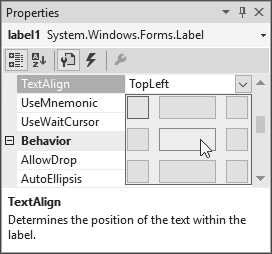
\includegraphics[width=0.95\textwidth,height=0.60\textheight,keepaspectratio]{images/fig2_28_centering_label.png}\\[1mm]
      \scriptsize \textbf{Hình 2.28:} Lựa chọn MiddleCenter trên lưới thuộc tính TextAlign (Deitel, trang 21).
    \end{column}
  \end{columns}
\end{frame}

% ==============================================================================
% SLIDE 38: BƯỚC 7: THÊM PICTUREBOX & CĂN CHỈNH BẰNG SNAP LINES
% ==============================================================================
\begin{frame}{Bước 7: Thêm Điều khiển PictureBox \& Đường Căn Snap Lines}
  \begin{columns}[T]
    \begin{column}{0.48\textwidth}
      \begin{block}{\textbf{Đường căn thông minh (Snap Lines):}}
        \begin{itemize}\small
          \item Kéo thả điều khiển \textbf{PictureBox} từ Toolbox đặt vào vùng trống bên dưới Label.
          \item Trong lúc kéo rê, Visual Studio tự động hiển thị các đường kẻ màu xanh dương (Snap lines) chỉ báo khoảng cách tiêu chuẩn giữa điều khiển với viền Form và các điều khiển lân cận.
          \item Giúp giao diện ứng dụng luôn gọn gàng, chuẩn thẩm mỹ mà không cần đo đạc thủ công.
        \end{itemize}
      \end{block}
    \end{column}

    \begin{column}{0.48\textwidth}
      \centering
      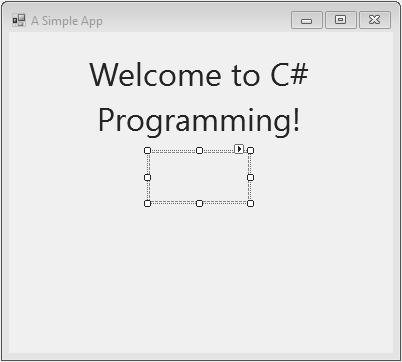
\includegraphics[width=0.95\textwidth,height=0.60\textheight,keepaspectratio]{images/fig2_29_inserting_picturebox.png}\\[1mm]
      \scriptsize \textbf{Hình 2.29:} Căn chỉnh PictureBox bằng đường Snap Lines (Deitel, trang 21).
    \end{column}
  \end{columns}
\end{frame}

% ==============================================================================
% SLIDE 39: BƯỚC 8: NẠP ẢNH TÀI NGUYÊN (SELECT RESOURCE DIALOG)
% ==============================================================================
\begin{frame}{Bước 8: Nạp Hình ảnh Tài nguyên (Select Resource Dialog)}
  \begin{columns}[T]
    \begin{column}{0.48\textwidth}
      \begin{block}{\textbf{Quy trình nhúng ảnh vào dự án:}}
        \begin{itemize}\small
          \item Chọn PictureBox $\to$ tìm thuộc tính \textbf{Image} trong Properties Window.
          \item Nhấp nút \textbf{\texttt{[...]}} để mở hộp thoại \textbf{Select Resource}.
          \item Chọn tùy chọn \textbf{Project resource file} để đóng gói ảnh vĩnh viễn vào tệp thực thi \texttt{.exe}.
          \item Nhấn nút \textbf{Import...} $\to$ duyệt chọn tệp hình ảnh linh vật \texttt{bug.png} từ thư mục tài nguyên.
          \item Nhấn \textbf{OK} để hoàn tất gán ảnh.
        \end{itemize}
      \end{block}
    \end{column}

    \begin{column}{0.48\textwidth}
      \centering
      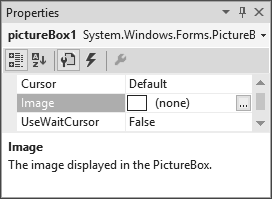
\includegraphics[width=0.85\textwidth,height=0.28\textheight,keepaspectratio]{images/fig2_30_picturebox_image_prop.png}\\[1mm]
      \scriptsize \textbf{Hình 2.30:} Thuộc tính Image của PictureBox (Deitel, trang 22).\\[2mm]
      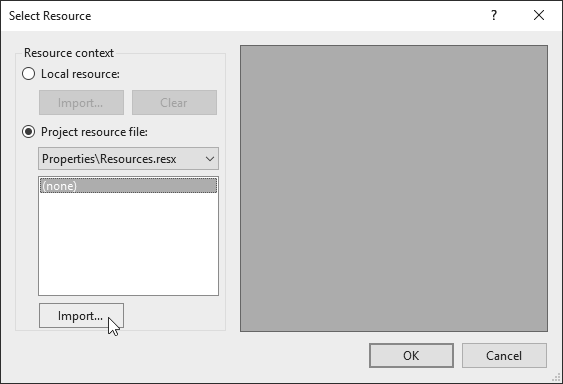
\includegraphics[width=0.85\textwidth,height=0.28\textheight,keepaspectratio]{images/fig2_31_select_resource_dialog.png}\\[1mm]
      \scriptsize \textbf{Hình 2.31:} Hộp thoại Select Resource (Deitel, trang 22).
    \end{column}
  \end{columns}
\end{frame}

% ==============================================================================
% SLIDE 40: BƯỚC 9: THUỘC TÍNH SIZEMODE CỦA PICTUREBOX
% ==============================================================================
\begin{frame}{Bước 9: Co giãn Hình ảnh với Thuộc tính SizeMode}
  \begin{columns}[T]
    \begin{column}{0.5\textwidth}
      \begin{block}{\textbf{Vấn đề thường gặp:}}
        Kích thước ảnh gốc thường lớn hơn khung PictureBox, khiến ảnh bị cắt xén (chỉ thấy một góc nhỏ).
      \end{block}

      \begin{exampleblock}{\textbf{Các giá trị của thuộc tính SizeMode:}}
        \begin{itemize}\footnotesize
          \item \textbf{Normal (mặc định):} Đặt ảnh ở góc trên bên trái, phần thừa bị cắt.
          \item \textbf{StretchImage:} Co/giãn ảnh vừa khít toàn bộ chiều rộng và chiều cao của khung PictureBox.
          \item \textbf{AutoSize:} Khung PictureBox tự phình to bằng đúng kích thước ảnh gốc.
          \item \textbf{CenterImage:} Căn ảnh vào chính giữa khung PictureBox.
          \item \textbf{Zoom:} Co giãn ảnh vừa khung nhưng giữ nguyên tỷ lệ khung hình (\textit{Aspect Ratio}) không bị méo.
        \end{itemize}
      \end{exampleblock}
    \end{column}

    \begin{column}{0.48\textwidth}
      \centering
      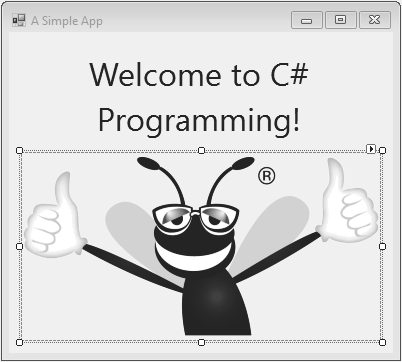
\includegraphics[width=0.85\textwidth,height=0.28\textheight,keepaspectratio]{images/fig2_33_scaling_image.png}\\[1mm]
      \scriptsize \textbf{Hình 2.33:} Chọn chế độ StretchImage (Deitel, trang 23).\\[2mm]
      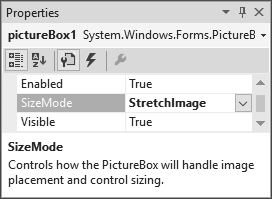
\includegraphics[width=0.85\textwidth,height=0.28\textheight,keepaspectratio]{images/fig2_34_picturebox_displaying.png}\\[1mm]
      \scriptsize \textbf{Hình 2.34:} Hình ảnh hiển thị hoàn hảo vừa vặn khung (Deitel, trang 23).
    \end{column}
  \end{columns}
\end{frame}

% ==============================================================================
% SLIDE 41: BƯỚC 10: BIÊN DỊCH, CHẠY THỬ & PHÂN BIỆT DESIGN VS RUN MODE
% ==============================================================================
\begin{frame}{Bước 10: Chạy Ứng dụng \& Phân biệt Design vs Run Mode}
  \begin{columns}[T]
    \begin{column}{0.48\textwidth}
      \begin{block}{\textbf{Khởi chạy ứng dụng:}}
        \begin{itemize}\small
          \item Nhấn \textbf{F5} (hoặc nút Start màu xanh lá trên toolbar).
          \item IDE chuyển từ \textbf{Design Mode} sang \textbf{Run Mode}.
          \item Cửa sổ ứng dụng \texttt{ASimpleApp} xuất hiện ở tiền cảnh (foreground), chạy mượt mà độc lập.
        \end{itemize}
      \end{block}

      \begin{tcolorbox}[colback=UniLightBlue!30,colframe=UniBlue,title=\textbf{Đặc trưng trạng thái Run Mode:},fonttitle=\small\bfseries]
        \footnotesize Trong lúc ứng dụng đang chạy, hầu hết các công cụ thiết kế trên Toolbox và Form Designer bị mờ (disabled) để bảo vệ tính toàn vẹn của mã nguồn.
      \end{tcolorbox}
    \end{column}

    \begin{column}{0.48\textwidth}
      \centering
      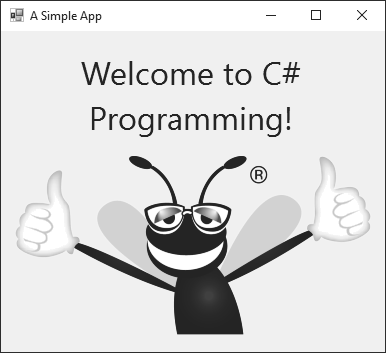
\includegraphics[width=0.95\textwidth,height=0.60\textheight,keepaspectratio]{images/fig2_35_ide_run_mode.png}\\[1mm]
      \scriptsize \textbf{Hình 2.35:} Visual Studio IDE ở chế độ Run Mode (Giáo trình Deitel, trang 24).
    \end{column}
  \end{columns}
\end{frame}

% ==============================================================================
% SLIDE 42: HANDS-ON LAB 3 - HOÀN THIỆN ỨNG DỤNG `ASimpleApp`
% ==============================================================================
\begin{frame}{Hands-on Lab 3: Xây dựng Hoàn thiện `ASimpleApp` (20 Phút)}
  \begin{columns}[T]
    \begin{column}{0.48\textwidth}
      \begin{tcolorbox}[colback=UniGreen!5,colframe=UniGreen,title=\textbf{NHIỆM VỤ THỰC HÀNH CÁ NHÂN:},fonttitle=\small\bfseries]
        \begin{enumerate}\small
          \item Tự thực hiện trọn vẹn 10 bước đã học trên máy tính phòng máy.
          \item Tạo Form có tiêu đề \texttt{"A Simple App"}, màu nền \texttt{LightCyan}.
          \item Thêm Label có chữ \texttt{"Welcome to Visual C\#!"}, Font Segoe UI 24pt Bold, căn lề \texttt{MiddleCenter}.
          \item Thêm PictureBox hiển thị hình ảnh tự chọn từ máy tính, thiết lập \texttt{SizeMode = StretchImage}.
          \item Nhấn \textbf{F5} chạy thử, kiểm tra căn lề và độ sắc nét.
          \item Gọi giảng viên chấm điểm thực hành tại chỗ.
        \end{enumerate}
      \end{tcolorbox}
    \end{column}

    \begin{column}{0.48\textwidth}
      \begin{tcolorbox}[colback=UniNavy!5,colframe=UniNavy,title=\textbf{TIÊU CHÍ ĐÁNH GIÁ (RUBRICS):},fonttitle=\small\bfseries]
        \begin{itemize}\small
          \item \textbf{Đúng bố cục (40\%):} Label ở trên, PictureBox ở dưới cân đối.
          \item \textbf{Thuộc tính chuẩn (40\%):} Đúng màu \texttt{LightCyan}, font 24pt bold, ảnh vừa khít không bị cắt xén méo mó.
          \item \textbf{Tác phong chuyên nghiệp (20\%):} Lưu trữ dự án đúng cấu trúc thư mục quy định, thao tác phím tắt nhanh nhẹn.
        \end{itemize}
      \end{tcolorbox}
    \end{column}
  \end{columns}
\end{frame}

% ==============================================================================
% SLIDE 43: CHECKPOINT 3 & TỔNG KẾT CHUẨN ĐẦU RA
% ==============================================================================
\begin{frame}{Checkpoint 3 \& Đánh giá Checklist Chuẩn Đầu Ra (CLOs)}
  \begin{columns}[T]
    \begin{column}{0.48\textwidth}
      \begin{alertblock}{\textbf{Câu hỏi Checkpoint 3:}}
        Khi muốn hình ảnh hiển thị trong PictureBox tự động co giãn để vừa khít hoàn toàn khung điều khiển, ta thiết lập thuộc tính \texttt{SizeMode} mang giá trị nào?
        \begin{enumerate}[(A)]
          \item \texttt{Normal}
          \item \texttt{AutoSize}
          \item \texttt{StretchImage}
          \item \texttt{CenterImage}
        \end{enumerate}
      \end{alertblock}
      \pause
      \footnotesize \textbf{Đáp án đúng: C (\texttt{StretchImage})}. Giá trị này ép ảnh co giãn theo đúng kích thước khung hình.
    \end{column}

    \begin{column}{0.48\textwidth}
      \begin{exampleblock}{\textbf{Checklist Chuẩn Đầu Ra Buổi học:}}
        \begin{itemize}\footnotesize
          \item[$\boxtimes$] \textbf{CLO 2.1:} Hiểu rõ bản chất IDE \& RAD.
          \item[$\boxtimes$] \textbf{CLO 2.2:} Phân biệt cấu trúc \texttt{.sln}, \texttt{.csproj}, \texttt{Form.cs}, \texttt{Form.Designer.cs}.
          \item[$\boxtimes$] \textbf{CLO 2.3:} Sử dụng thành thạo Menus, Toolbars và phím tắt (F5, F4, Ctrl+Shift+S).
          \item[$\boxtimes$] \textbf{CLO 2.4:} Làm chủ Solution Explorer, Toolbox và Properties Window.
          \item[$\boxtimes$] \textbf{CLO 2.5:} Tự tay xây dựng thành công ứng dụng GUI hoàn chỉnh có văn bản và hình ảnh.
        \end{itemize}
      \end{exampleblock}
    \end{column}
  \end{columns}
\end{frame}

% ==============================================================================
% SLIDE 44: BÀI TẬP VỀ NHÀ - THỬ THÁCH THIẾT KẾ 5 GIAO DIỆN THỰC TẾ
% ==============================================================================
\begin{frame}{Bài tập Về Nhà: Thử thách Thiết kế 5 Giao diện Thực tế}
  \begin{columns}[T]
    \begin{column}{0.48\textwidth}
      \textbf{Nhiệm vụ tự học (Giáo trình Deitel, trang 29--31):}
      \begin{enumerate}\footnotesize
        \item \textbf{Bài 2.7 (Stop Watch GUI):} Thiết kế giao diện Đồng hồ bấm giờ có các nút Start, Stop, Reset (Hình 2.36).
        \item \textbf{Bài 2.8 (Login Form GUI):} Thiết kế màn hình Đăng nhập có Username, Password, CheckBox Remember (Hình 2.37).
        \item \textbf{Bài 2.9 (Calculator GUI):} Thiết kế bàn phím Máy tính bỏ túi với lưới các nút số 0--9 và phép tính (Hình 2.38).
        \item \textbf{Bài 2.10 (Alarm Clock GUI):} Thiết kế giao diện Đồng hồ báo thức hẹn giờ (Hình 2.39).
        \item \textbf{Bài 2.11 (Radio GUI):} Thiết kế máy nghe đài Radio có dò kênh và chỉnh âm lượng (Hình 2.40).
      \end{enumerate}
    \end{column}

    \begin{column}{0.48\textwidth}
      \centering
      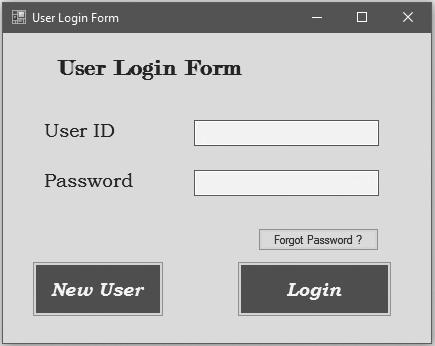
\includegraphics[width=0.85\textwidth,height=0.28\textheight,keepaspectratio]{images/fig2_37_login_form_gui.png}\hspace{2mm}
      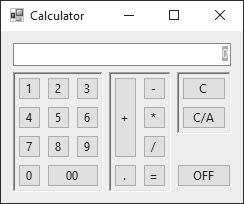
\includegraphics[width=0.85\textwidth,height=0.28\textheight,keepaspectratio]{images/fig2_38_calculator_gui.png}\\[2mm]
      \scriptsize \textbf{Hình 2.37 \& 2.38:} Giao diện Màn hình Đăng nhập và Máy tính bỏ túi.\\[3mm]
      \begin{tcolorbox}[colback=UniGreen!10,colframe=UniGreen,title=\textbf{Chuẩn bị cho Chương 3:},fonttitle=\small\bfseries]
        \footnotesize Đọc trước Chương 3: \textit{Introduction to C\# App Programming} -- Bắt đầu viết mã lệnh xử lý số học, biến số và điều khiển luồng!
      \end{tcolorbox}
    \end{column}
  \end{columns}
\end{frame}

\end{document}
